\subsection{Введение}

Чтобы понять, при каком значении сопротивления в цепи будет наблюдаться \textbf{колебательный} процесс, а при каком \textbf{апериодический}, нужно найти характеристическое сопротивление, которое для цепи второго порядка определяется как:

\[
	p = \sqrt{\frac{L}{C}} = \sqrt{\frac{0,48}{300 \cdot 10^{-6}}} = 40 \, \text{Ом}
\]

На основе этой величины можно понять какой будет процесс: Если $R > p$, то затухания колебаний ускоряются и энергия системы не возвращается в исходное состояние, если $R = 2 \cdot p$ -- это критический момент, когда процесс перестаёт быть апериодическим, но возвращается в равновесное состояние без колебаний, а при $R < 2 \cdot p$ энергия будет поочерёдно передаваться между индуктивностью и ёмкостью, вызывая затухающие колебания.

Таким образом, при $R = 4 \cdot p = 4 \cdot 40 = 160 \, \text{Ом}$ наблюдается \textit{апериодический} процесс, а при $R = \frac{p}{2} = \frac{40}{2} = 20 \, \text{Ом}$ -- \textit{колебательный}.


% -------------------------------


\subsection{Исследование апериодического процесса}

\subsubsection{Схема исследуемой цепи}
На рисунке 3 представлена схема замещения цепи второго порядка, состоящей из генератора прямоугольного напряжения с резистивной, ёмкостной и индуктивной нагрузками, созданная в приложении LTspice.

\begin{figure}[H]
	\centering
	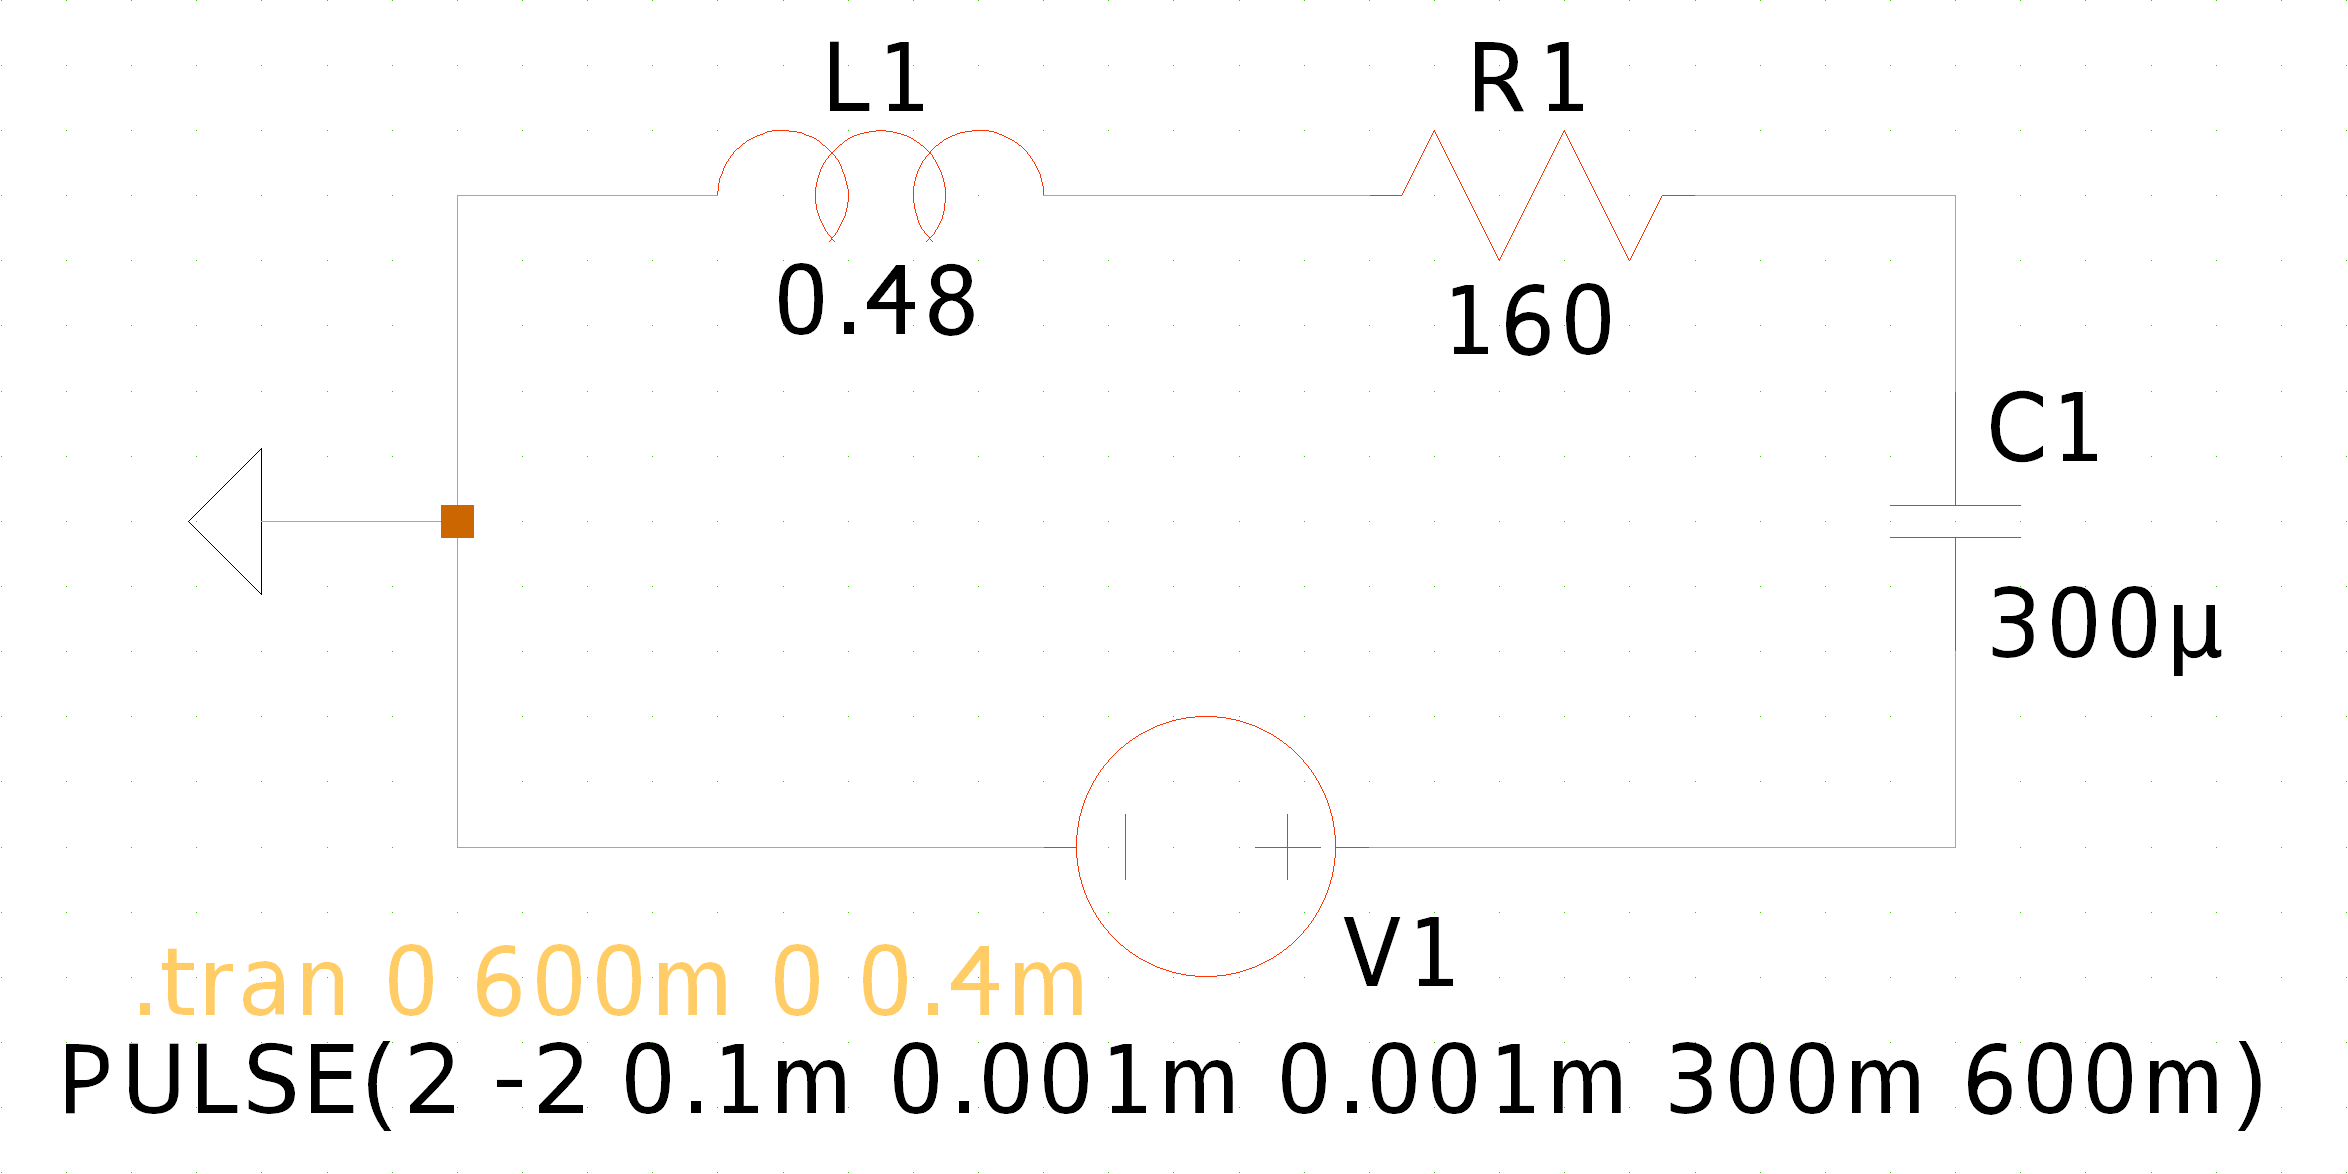
\includegraphics[width=1\textwidth]{./data/rcl_1-schema.png}
	\caption{Схема замещения RCL-цепи в LTspice.}
\end{figure}

\subsubsection{Расчётные формулы и расчёты}

Значение времени переходного процесса \( t_{0.5} \) определяется как время, за которое напряжение на конденсаторе достигает половины своего установившегося значения. Постоянная времени \( \tau \) определяется как:

\[
	\tau = \frac{t_{0.5}}{\ln 2}
\]

\textbf{Вычисление постоянной времени \( \tau \):}

\[
	\tau = \frac{t_{0.5}}{\ln 2} = \frac{8.41833 \, \text{мс}}{0.69314718} = 12.144 \, \text{мс}
\]

\subsubsection{График апериодического переходного процесса}
% time	V(N003,N001)  V(n002)  V(n003)  I(C1)

\begin{figure}[H]
	\centering
	\begin{tikzpicture}[scale=0.88]
		\begin{axis}[
				width=17cm, height=12cm,
				xlabel={Time [ms]},    % X-axis label
				ylabel={Voltage [V]},    % Y-axis label
				grid=major,           % Enable grid
				legend style={at={(0.857,0.95)}, anchor=north west}, % Legend position
				thick,                % Line thickness
				xmin=0, xmax=600,    % X-axis range
				ymin=-4, ymax=4,      % Y-axis range
				axis y line=left,
				axis x line=bottom,
				label style={font=\small},
				tick label style={font=\small},
				major tick length=0.2cm,
				ytick style={thick, black},
				xtick style={thick, black},
				ytick={-3.2, -2.4, -1.6, -0.8, 0, 0.8, 1.6, 2.4, 3.2},
				extra y ticks={-4, 4},
				extra y tick style={tick style={opacity=0}},
				x unit=0.001,
			]

			% Plot V(n001)
			\addplot[
				color=red,
				thick,
			] table [x expr=\thisrowno{0}*1000, y index=3, col sep=space] {./data/lab2-3.txt};
			\addlegendentry{$E$}

			% Plot V(n002)
			\addplot[
				color=magenta,
				thick,
			] table [x expr=\thisrowno{0}*1000, y index=1, col sep=space] {./data/lab2-3.txt};
			\addlegendentry{$U_L$}
			%
			% \addplot[color=black, only marks, mark=*, mark size=1pt] coordinates {(0, 4)};
			% \node[anchor=west] at (axis cs:0,3.85) {\scriptsize $U_L(0+) = 4 \, V$};
			%
			% \addplot[color=black, only marks, mark=*, mark size=1.5pt] coordinates {(60, 0.027)};
			% \node[anchor=east] at (axis cs:61,-0.15) {\scriptsize $0.027 \, V = U_L(\infty)$};
			% \draw[dashed, grey, very thin] (axis cs:0, 0.027) -- (axis cs:60, 0.027);

			% Plot V(n002)
			\addplot[
				color=green,
				thick,
				% nodes near coords,
				% mark=*,
				% every node near coord/.append style={font=\tiny, black}
			] table [x expr=\thisrowno{0}*1000, y index=2, col sep=space] {./data/lab2-3.txt};
			\addlegendentry{$U_c$}

			% \draw[dashed,grey,very thin] (axis cs:120,1.972884) -- (axis cs:60.1,1.972884);
			% \addplot[color=black, only marks, mark=*, mark size=1.5pt] coordinates {(60.1,1.972884)};
			% \node[anchor=west] at (axis cs:60.1,1.872884) {\scriptsize $U_c(\infty) = 1.973 \, V$};
			%
			% \draw[dashed,grey,very thin] (axis cs:120,-1.973) -- (axis cs:120, -1.973)
			% \addplot[color=black, only marks, mark=*, mark size=1.5pt] coordinates {(120, -1.973)};
			% \node[anchor=east] at (axis cs:121,-1.82) {\scriptsize $ -1.973 \, V = U_c(0+)$};


		\end{axis}

		% Secondary axis for Current
		\begin{axis}[
				width=17cm, height=12cm,
				xmin=0, xmax=600,    % X-axis range (same as for Voltage)
				ymin=-80, ymax=80,  % Y-axis range for Current
				axis y line=right,         % Place this axis on the right for Current
				axis x line=none,
				thick,
				ylabel={Current [mA]}, % Y-axis label for Current
				label style={font=\small},
				tick label style={font=\small},
				major tick length=0.2cm,
				ytick style={thick, black},
				ytick={-70, -60, -50, -40, -30, -20, -10, 0, 10, 20, 30, 40, 50, 60, 70},
				extra y ticks={-80, 80},
				extra y tick style={tick style={opacity=0}},
				legend style={at={(0.961,0.765)}, anchor=north east},
			]
			% Plot I
			\addplot[
				color=cyan,
				thick,
			] table [x expr=\thisrowno{0}*1000, y expr=\thisrowno{4}*1000, col sep=space] {./data/lab2-3.txt};
			\addlegendentry{$I$}

			% \addplot[color=black, only marks, mark=*, mark size=1.5pt] coordinates {(120, -49.324)};
			% \node[
			% 	anchor=east,
			% 	font=\scriptsize
			% ] at (axis cs:121,-47) {$-49.324\, \text{mA} = I(0+)$};
			%
			% \addplot[color=black, only marks, mark=*, mark size=1.5pt] coordinates {(60.1, 49.325)};
			% \draw[dashed, grey, very thin] (axis cs:60, 49.3) -- (axis cs:120, 49.3);
			% \node[anchor=west] at (axis cs:60.1,47) {\scriptsize $I(\infty) = 49.325 \, mA$};
		\end{axis}
	\end{tikzpicture}
\end{figure}


\subsubsection{Таблица результатов 4.4}


% -------------------------------


\subsection{Исследование колебательного процесса}

\subsubsection{Схема исследуемой цепи}
На рисунке 4 представлена схема замещения генератора прямоугольного напряжения с резистивной, ёмкостной и индуктивной нагрузками, созданная в приложении LTspice.

\begin{figure}[H]
	\centering
	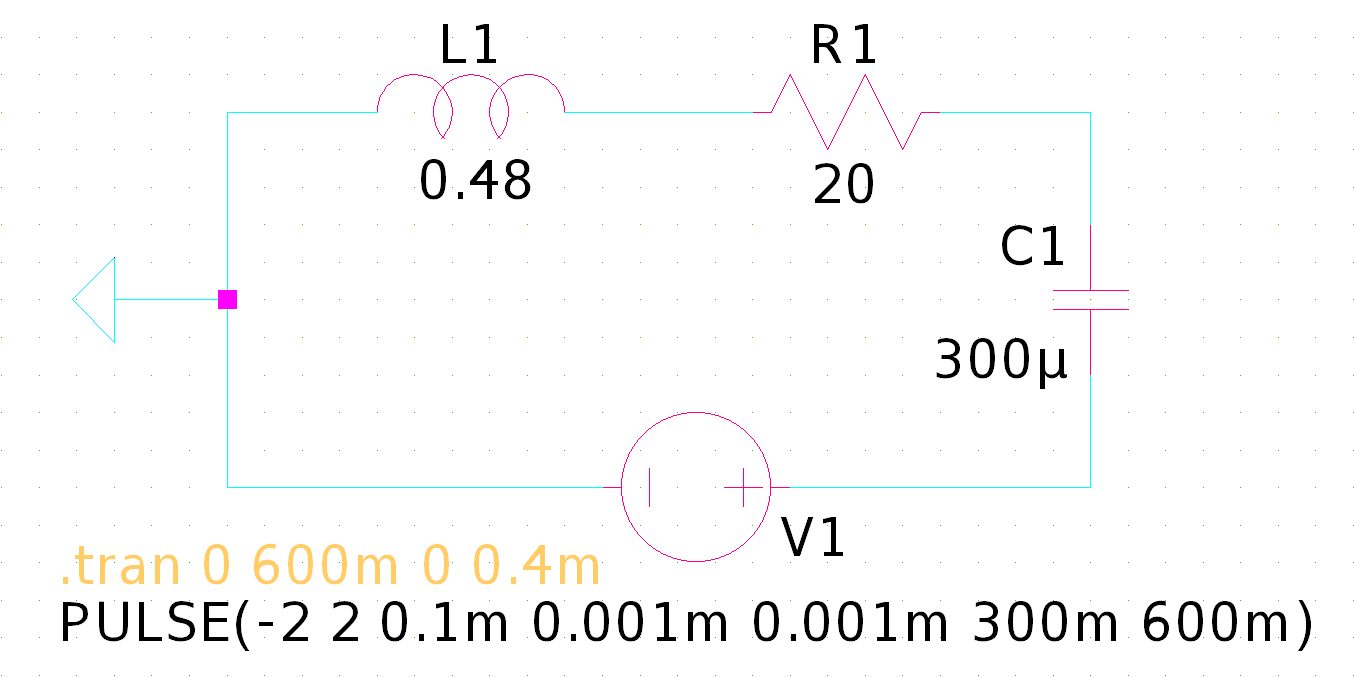
\includegraphics[width=0.96\textwidth]{./data/rcl_2-schema.png}
	\caption{Схема замещения RCL-цепи в LTspice.}
\end{figure}

\subsubsection{Расчётные формулы и расчёты}

\subsubsection{График колебательного переходного процесса}
% time	V(N003,N001)  V(n002)  V(n003)  I(C1)

\begin{figure}[H]
	\centering
	\begin{tikzpicture}[scale=0.88]
		\begin{axis}[
			width=17cm, height=12cm,
			xlabel={Время [мс]},
			ylabel={Напряжение [В]},
			grid=major,           % Enable grid
			legend style={at={(0.857,0.95)}, anchor=north west}, % Legend position
			thick,                % Line thickness
			xmin=0, xmax=600,    % X-axis range
			ymin=-4, ymax=4,      % Y-axis range
			axis y line=left,
			axis x line=bottom,
			label style={font=\small},
			tick label style={font=\small},
			major tick length=0.2cm,
			ytick style={thick, black},
			xtick style={thick, black},
			ytick={-3, -2, -1, 0, 1, 2, 3},
			extra y ticks={-4, 4},
			extra y tick style={tick style={opacity=0}},
			x unit=0.001,
			]

			% Plot V(n001)
			\addplot[
				color=teal,
				line width=1.2pt,
			] table [x expr=\thisrowno{0}*1000, y index=3, col sep=space] {./data/lab2-4.txt};
			\addlegendentry{$E$}

			% Plot V(n002)
			\addplot[
				color=orange,
				line width=1.2pt,
			] table [x expr=\thisrowno{0}*1000, y index=1, col sep=space] {./data/lab2-4.txt};
			\addlegendentry{$U_c$}
			%
			% \addplot[color=black, only marks, mark=*, mark size=1pt] coordinates {(0, 4)};
			% \node[anchor=west] at (axis cs:0,3.85) {\scriptsize $U_L(0+) = 4 \, V$};
			%
			% \addplot[color=black, only marks, mark=*, mark size=1.5pt] coordinates {(60, 0.027)};
			% \node[anchor=east] at (axis cs:61,-0.15) {\scriptsize $0.027 \, V = U_L(\infty)$};
			% \draw[dashed, grey, very thin] (axis cs:0, 0.027) -- (axis cs:60, 0.027);

			% Plot V(n002)
			\addplot[
				color=magenta,
				line width=1.2pt,
				% nodes near coords,
				% mark=*,
				% every node near coord/.append style={font=\tiny, black}
			] table [x expr=\thisrowno{0}*1000, y index=2, col sep=space] {./data/lab2-4.txt};
			\addlegendentry{$U_L$}

			% \draw[dashed,grey,very thin] (axis cs:120,1.972884) -- (axis cs:60.1,1.972884);
			% \addplot[color=black, only marks, mark=*, mark size=1.5pt] coordinates {(60.1,1.972884)};
			% \node[anchor=west] at (axis cs:60.1,1.872884) {\scriptsize $U_c(\infty) = 1.973 \, V$};
			%
			% \draw[dashed,grey,very thin] (axis cs:120,-1.973) -- (axis cs:120, -1.973)
			% \addplot[color=black, only marks, mark=*, mark size=1.5pt] coordinates {(120, -1.973)};
			% \node[anchor=east] at (axis cs:121,-1.82) {\scriptsize $ -1.973 \, V = U_c(0+)$};


		\end{axis}

		% Secondary axis for Current
		\begin{axis}[
			width=17cm, height=12cm,
			xmin=0, xmax=600,    % X-axis range (same as for Voltage)
			ymin=-80, ymax=80,  % Y-axis range for Current
			axis y line=right,         % Place this axis on the right for Current
			axis x line=none,
			thick,
			line width=1.3pt,
			ylabel={Ток [мА]},
			label style={font=\small},
			tick label style={font=\small},
			major tick length=0.2cm,
			ytick style={thick, black},
			ytick={-60, -40, -20, 0, 20, 40, 60},
			extra y ticks={-80, 80},
			extra y tick style={tick style={opacity=0}},
			legend style={at={(0.961,0.765)}, anchor=north east},
			]
			% Plot I
			\addplot[
				color=cyan,
				line width=1.2pt,
			] table [x expr=\thisrowno{0}*1000, y expr=\thisrowno{4}*1000, col sep=space] {./data/lab2-4.txt};
			\addlegendentry{$I$}

			% \addplot[color=black, only marks, mark=*, mark size=1.5pt] coordinates {(120, -49.324)};
			% \node[
			% 	anchor=east,
			% 	font=\scriptsize
			% ] at (axis cs:121,-47) {$-49.324\, \text{mA} = I(0+)$};
			%
			% \addplot[color=black, only marks, mark=*, mark size=1.5pt] coordinates {(60.1, 49.325)};
			% \draw[dashed, grey, very thin] (axis cs:60, 49.3) -- (axis cs:120, 49.3);
			% \node[anchor=west] at (axis cs:60.1,47) {\scriptsize $I(\infty) = 49.325 \, mA$};
		\end{axis}
	\end{tikzpicture}
\end{figure}


\subsubsection{Таблица результатов 4.5}

\subsection{Выводы по второй части}
